\begin{figure}[htbp]
\begin{center}
\iffastcompile
    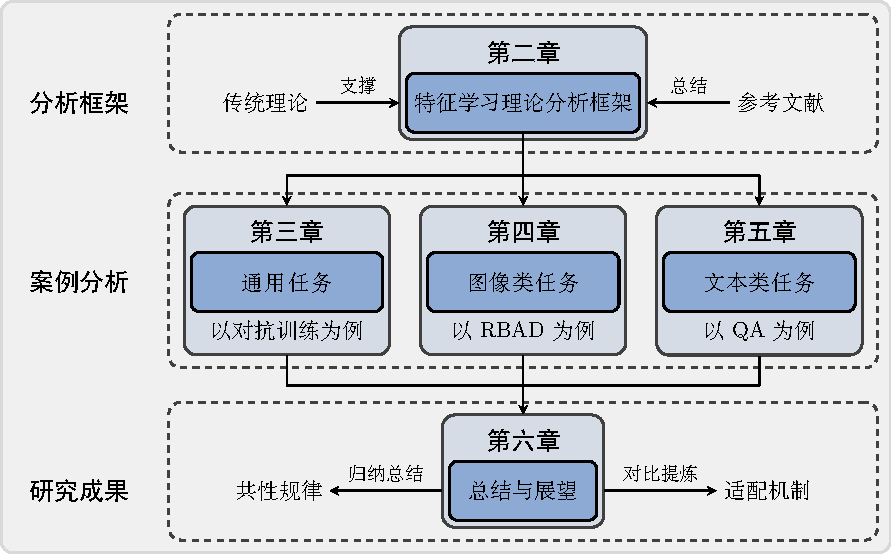
\includegraphics[width=0.99\textwidth]{figures/tikz/research_roadmap.pdf}
\else
    \begin{tikzpicture}[node distance=2cm]
        % 分析框架
        \node (top) [block] {特征学习理论分析框架};
        \node (top_caption) [above] at (top.north) {\zihao{-4}\heiti{第二章}};
        \begin{pgfonlayer}{bg3}
            \node (top_box) [draw=darkgray, fill=blue-background, line width=1pt, rounded corners=6pt, inner sep=0.1cm, fit=(top_caption) (top)] {};
        \end{pgfonlayer}
        \node (theory) [left] at ([xshift=-1.5cm]top.west) {传统理论};
        \node (ref) [right] at ([xshift=1.5cm]top.east) {参考文献};
        \draw [arrow] (theory.east) -- (top_box.west |- theory.east) node [above, midway] {\zihao{-5} 支撑};
        \draw [arrow] (ref.west) -- (top_box.east |- ref.west) node [above, midway] {\zihao{-5} 总结};
        \begin{pgfonlayer}{bg2}
            \node (topbox) [draw=darkgray, dashed, line width=1pt, rounded corners=6pt, inner sep=0.2cm, minimum width=12cm, align=center, fit=(theory) (top_box) (ref)] {};
        \end{pgfonlayer}

        % 案例分析
        \node (mid1) [block, below=of top, xshift=-4cm, text width=3cm] {通用任务};
        \node (mid1_caption) [above] at (mid1.north) {\zihao{-4}\heiti{第三章}};
        \node (mid1_task) [below] at (mid1.south) {以对抗训练为例};
        \begin{pgfonlayer}{bg3}
            \node (mid1_box) [draw=darkgray, fill=blue-background, line width=1pt, rounded corners=6pt, inner sep=0.1cm, fit=(mid1_caption) (mid1) (mid1_task)] {};
        \end{pgfonlayer}
        \node (mid2) [block, below=of top, text width=3cm] {图像类任务};
        \node (mid2_caption) [above] at (mid2.north) {\zihao{-4}\heiti{第四章}};
        \node (mid2_task) [below] at (mid2.south) {以RBAD为例};
        \begin{pgfonlayer}{bg3}
            \node (mid2_box) [draw=darkgray, fill=blue-background, line width=1pt, rounded corners=6pt, inner sep=0.1cm, fit=(mid2_caption) (mid2) (mid2_task)] {};
        \end{pgfonlayer}
        \node (mid3) [block, below=of top, xshift=4cm, text width=3cm] {文本类任务};
        \node (mid3_caption) [above] at (mid3.north) {\zihao{-4}\heiti{第五章}};
        \node (mid3_task) [below] at (mid3.south) {以QA为例};
        \begin{pgfonlayer}{bg3}
            \node (mid3_box) [draw=darkgray, fill=blue-background, line width=1pt, rounded corners=6pt, inner sep=0.1cm, fit=(mid3_caption) (mid3) (mid3_task)] {};
        \end{pgfonlayer}
    
        \begin{pgfonlayer}{bg2}
        \node (midbox) [draw=darkgray, dashed, line width=1pt, rounded corners=6pt, inner sep=0.2cm, minimum width=12cm, align=center, fit=(mid1_box) (mid2_box) (mid3_box)] {};
        \end{pgfonlayer}

        % 研究成果
        \node (bottom) [block, below=2.5cm of mid2] {总结与展望};
        \node (bottom_caption) [above] at (bottom.north) {\zihao{-4}\heiti{第六章}};
        \begin{pgfonlayer}{bg3}
            \node (bottom_box) [draw=darkgray, fill=blue-background, line width=1pt, rounded corners=6pt, inner sep=0.1cm, fit=(bottom_caption) (bottom)] {};
        \end{pgfonlayer}
        \node (modern_theory) [left] at ([xshift=-2cm]bottom.west) {共性规律};
        \node (application) [right] at ([xshift=2cm]bottom.east) {适配机制};
        \draw [arrow] (bottom_box.west |- modern_theory.east) -- (modern_theory.east) node [above, midway] {\zihao{-5} 归纳总结};
        \draw [arrow] (bottom_box.east |- application.west) -- (application.west) node [above, midway] {\zihao{-5} 对比提炼};
        \begin{pgfonlayer}{bg2}
            \node (bottombox) [draw=darkgray, dashed, line width=1pt, rounded corners=6pt, inner sep=0.2cm, minimum width=12cm, align=center, fit=(modern_theory) (bottom_box) (application)] {};
        \end{pgfonlayer}
    
        % 虚线框左上角加标题
        \coordinate (mid_caption) at ($(mid1.west) + (-3cm, 0)$);
        \coordinate (top_caption) at (mid_caption |- theory.west);
        \coordinate (bottom_caption) at (mid_caption |- bottom.west);
        \node (top_summary) [right, inner sep=2pt] at ([xshift=0.2cm]mid_caption) {\zihao{-4}\heiti{案例分析}};
        \node (mid_summary) [right, inner sep=2pt] at ([xshift=0.2cm]top_caption) {\zihao{-4}\heiti{分析框架}};
        \node (bottom_summary) [right, inner sep=2pt] at ([xshift=0.2cm]bottom_caption) {\zihao{-4}\heiti{研究成果}};
    
        % 第一层 -> 第二层
        \coordinate (mid_branch) at ($(mid2_box.north) + (0, 0.5cm)$);
        \coordinate (mid_branch_left) at ($(mid1_box.north) + (0, 0.5cm)$);
        \coordinate (mid_branch_right) at ($(mid3_box.north) + (0, 0.5cm)$);
        \draw [line] (top.south) -- (mid_branch);
        \draw [line] (mid_branch) -- (mid_branch_left);
        \draw [line] (mid_branch) -- (mid_branch_right);
        \draw [arrow] (mid_branch_left) -- (mid1_box.north);
        \draw [arrow] (mid_branch) -- (mid2_box.north);
        \draw [arrow] (mid_branch_right) -- (mid3_box.north);
    
        % 第二层 -> 第三层
        \coordinate (bottom_branch) at ($(mid2_box.south) + (0, -0.5cm)$);
        \coordinate (bottom_branch_left) at ($(mid1_box.south) + (0, -0.5cm)$);
        \coordinate (bottom_branch_right) at ($(mid3_box.south) + (0, -0.5cm)$);
        \draw [line] (mid1_box.south) -- (bottom_branch_left);
        \draw [line] (mid2_box.south) -- (bottom_branch);
        \draw [line] (mid3_box.south) -- (bottom_branch_right);
        \draw [line] (bottom_branch_left) -- (bottom_branch);
        \draw [line] (bottom_branch) -- (bottom_branch_right);
        \draw [arrow] (bottom_branch) -- (bottom_box.north);

        \begin{pgfonlayer}{bg1}
            \node (background) [draw=darkgray-background, fill=darkgray-background!40, line width=1pt, rounded corners=6pt, inner sep=0.2cm, minimum width=0.99\textwidth, align=center, fit=(topbox) (midbox) (bottombox) (mid_caption) (top_caption) (bottom_caption)] {};
        \end{pgfonlayer}
    \end{tikzpicture}
\fi
\end{center}
\end{figure}